\documentclass{beamer}
\usepackage{multirow}
\usepackage{booktabs}
\usepackage{graphicx}
\usepackage[backend=biber,
style=authoryear-comp]{biblatex}

\setbeamercovered{transparent}
\usetheme{Madrid}
\bibliography{sample.bib}

\title{\textbf{Discussion:} Systemic analysis: A method to show how funds flow through financial systems}
\author{\textbf{Author:} Juliaan Bol
\\
\textbf{Discussant:} Mateusz Dadej}

\date{ICMA Centre, University of Reading, June 2024
\\
Doctoral Finance Symposium}

% Removes icon in bibliography
%\setbeamertemplate{bibliography item}{}

\begin{document}

\titlepage

\begin{frame}{Overview}

\begin{itemize}
    \item<1-> The paper introduces a framework to analyze flow of funds through the financial system. 
    \item<2-> The system satisfy accounting conditions:
    \begin{itemize}
       \item<3-> $L_{fec}^t = A_{fec}^t$ (assets = liabilities)
       \item<4-> Complete balance sheet identity: $N_e^t + \sum_{i=1}^{l}(A_i^t + V_i^t) = \sum_{j=1}^{l} L_j^t + S_e^t$
    \end{itemize}    
    \item<5-> The flow of funds ($\Delta A_d$) can be disentangled into:
    \begin{itemize}
        \item<6->$\underbrace{\frac{A_t^d}{T_e^t} \left(\sum_{j \in P} \Delta_s L_j + \Delta_s S_e\right)}_{\text{Growth factors}} + \underbrace{\frac{1}{T_e^t} \sum_{i \in P}\left(A_i^t \Delta A_d - A_d^t \Delta A_i\right)}_{\text{Realocation factors}} + \frac{A_d^t}{T_e^t} \Delta R_e$
        
    \end{itemize}    
\end{itemize}    

\end{frame}    

\begin{frame}{System diagram}
    \begin{figure}[H]
        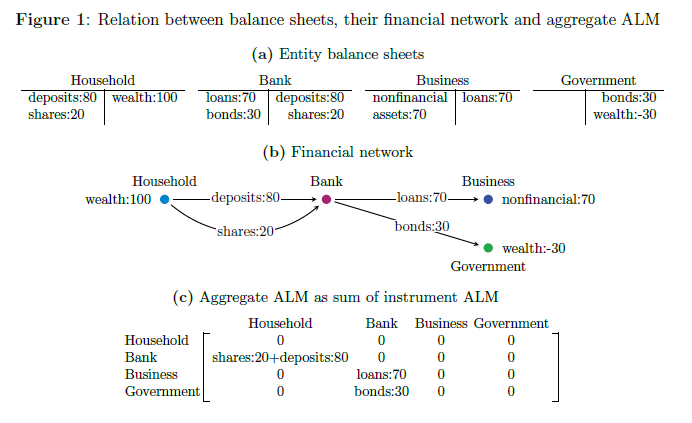
\includegraphics[scale=0.8]{diagram.png}
        \centering
    \end{figure}  
\end{frame}    

\begin{frame}{My take on the paper}
\begin{itemize}
    \item<1-> The framework is \textbf{very} general and broadly applicable. 
    \begin{itemize}
        \item<2-> Stress testing
        \item<3-> Policy scenario evaluation
        \item<4-> Systemic crisis analysis
    \end{itemize}
    \item<5-> Minimal amount of assumptions due to accounting relations.
    \item<6-> Ease of communicating results.
    
\end{itemize}
\end{frame}    

\begin{frame}{Suggestions, comments, etc...}
    \begin{itemize}
        \item<1-> Consider a simple VAR model with time-varying parameters for break point detection (à la \cite{deibold}) in order to have a single model for breaks and eliminate potential spurious breaks. Alternatively, graphical models.
        \item<2-> Regarding "Creating financial systems from national accounts": Consider matrix completion literature applied to interbank markets (e.g. \cite{anand18} for benchmark of various methods). 
        \item<3-> See the literature for stock-flow consistent modeling (\cite{godley})
        \item<4-> Consider the literature suggesting endogenous money/deposit creation (\cite{mcleay})
    \end{itemize}    
\end{frame}


\begin{frame}[allowframebreaks]
\frametitle{References}
  \printbibliography
\end{frame}

\end{document}